值得注意的是,由于openwrt的版本不同,实验指导书中的一些配置不再适用，如openwrt防火墙的配置
\begin{lstlisting}
list network 'lan1 lan2'
\end{lstlisting}
这里实验的时候发现总是ping不通,新版openwrt会把 lan1 lan2 当成一个网络名称。

此时应该分成两行：
\begin{lstlisting}
list network 'lan1'
list network 'lan2'
\end{lstlisting}
另一个值得注意的地方是，实验指导书有些自相矛盾的地方,实验1中要求tcpdump监测eth0
\begin{figure}[H]
    \centering
    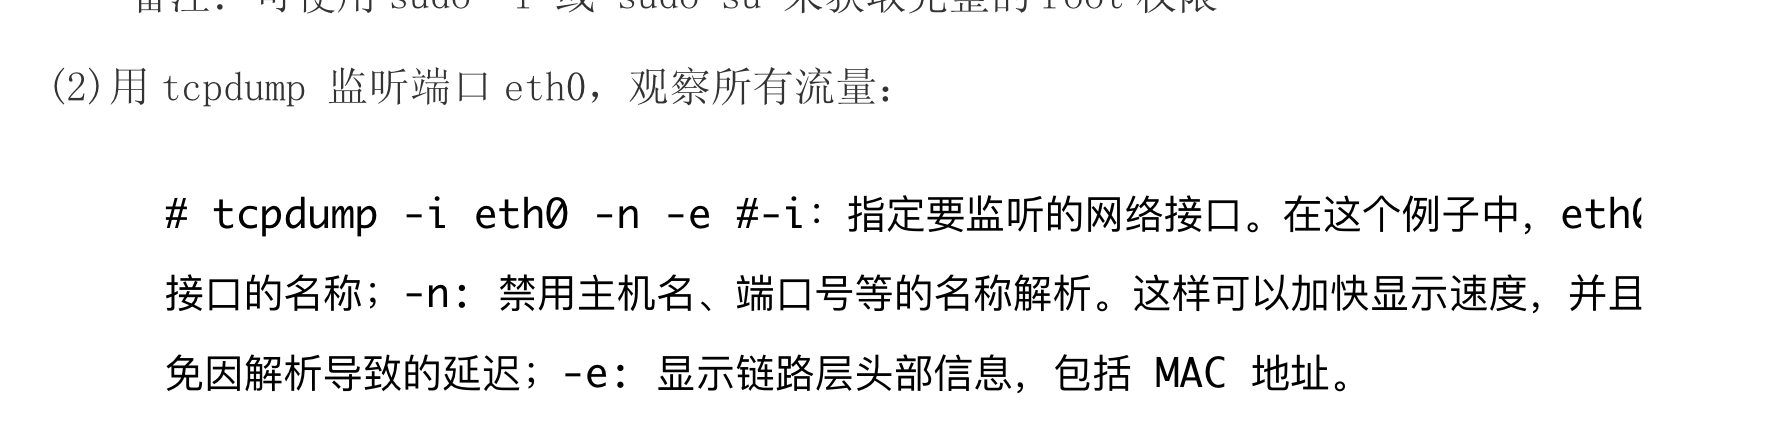
\includegraphics[width=0.8\textwidth]{figures/dis0.png}
    \caption{tcpdump监测eth0}
\end{figure}
但是在比较新的ubuntu版本中，网卡不再以eth0等命名,而是enp0s3,这在网络环境配置指导书里有
\begin{figure}[H]
    \centering
    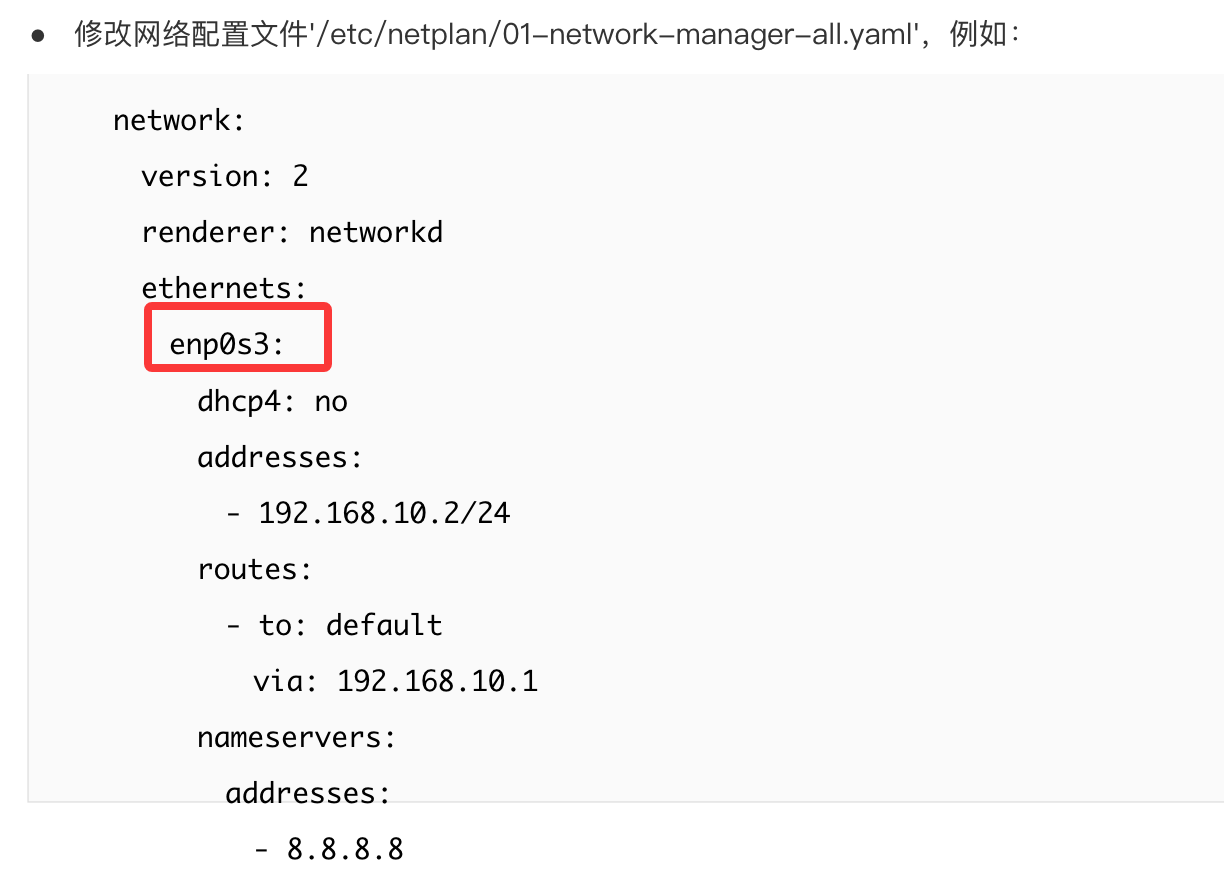
\includegraphics[width=0.8\textwidth]{figures/dis2.png}
    \caption{以enp0s3命名}
\end{figure}
可疑的是，实验指导书此处应当是使用docker做的，docker中的ubuntu可以直接命名网卡,此处显然会对采用virtualbox方案的同学产生误导
\begin{figure}[H]
    \centering
    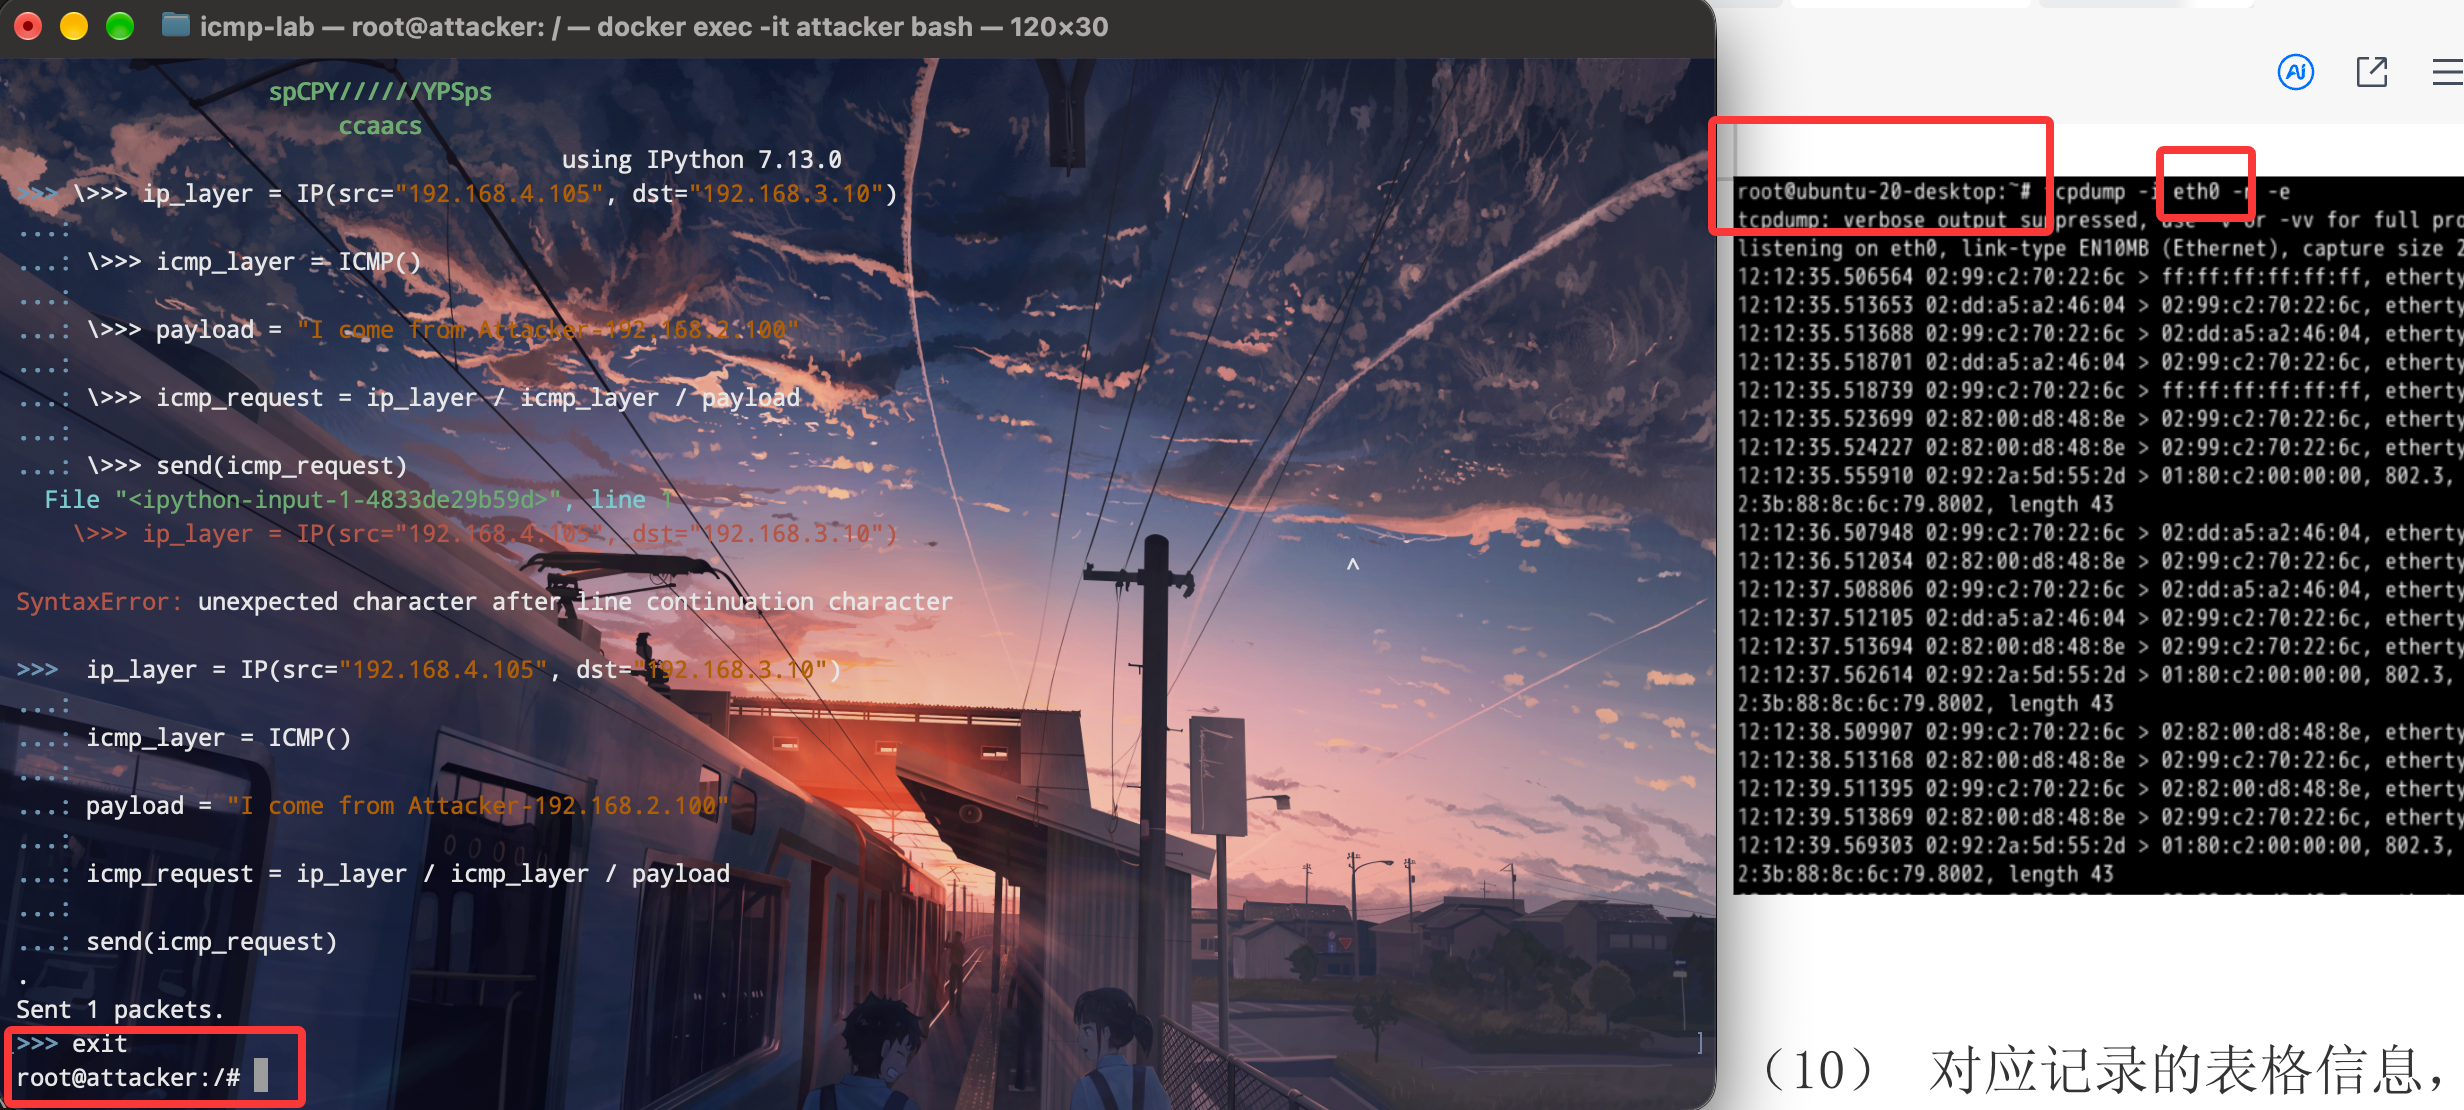
\includegraphics[width=0.8\textwidth]{figures/dis1.png}
    \caption{疑似docker}
\end{figure}